\chapter{Small oscillations-solutions}
\begin{abox}
	Practice set 1
\end{abox}
\begin{enumerate}
	\begin{minipage}{\textwidth}
		\item  A particle of unit mass moves in a potential $V(x)=a x^{2}+\frac{b}{x^{2}}$, where $a$ and $b$ are positive constants. The angular frequency of small oscillations about the minimum of the potential is
		\exyear{NET JUNE 2011}
	\end{minipage}
	\begin{tasks}(2)
		\task[\textbf{A.}] $\sqrt{8 b}$
		\task[\textbf{B.}]$\sqrt{8 a}$
		\task[\textbf{C.}] $\sqrt{8 a / b}$
		\task[\textbf{D.}]$\sqrt{8 b / a}$
	\end{tasks}
	\begin{answer}
		\begin{align*}
		V(x)&=a x^{2}+\frac{b}{x^{2}} \Rightarrow \frac{\partial V}{\partial x}=0 \Rightarrow 2 a x-\frac{2 b}{x^{3}}=0 \Rightarrow a x^{4}-b=0 \Rightarrow x_{0}=\left(\frac{b}{a}\right)^{\frac{1}{4}}\\
		\text { Since } \omega&=\sqrt{\frac{k}{m}}, m=1\\
		k&=\left.\frac{\partial^{2} V}{\partial x^{2}}\right|_{x=x_{0}} \text { where } x_{0} \text { is stable equilibrium point. }\\
		\text { Hence } k&=\frac{\partial^{2} V}{\partial x^{2}}=2 a+\frac{6 b}{x_{0}^{4}}=2 a+\frac{6 b}{b /}=8 a \text { at } x=x_{0}=\left(\frac{b}{a}\right)^{\frac{1}{4}}\\
		\text { Thus, } \omega&=\sqrt{8 a} \text {. }
		\end{align*}
		The correct option is \textbf{(b)}
	\end{answer}
	\begin{minipage}{\textwidth}
		\item Consider the motion of a classical particle in a one dimensional double-well potential $V(x)=\frac{1}{4}\left(x^{2}-2\right)^{2} .$ If the particle is displaced infinitesimally from the minimum on the $x$-axis (and friction is neglected), then
		\exyear{NET JUNE 2012}
	\end{minipage}
	\begin{tasks}(1)
		\task[\textbf{A.}] the particle will execute simple harmonic motion in the right well with an angular frequency $\omega=\sqrt{2}$
		\task[\textbf{B.}]the particle will execute simple harmonic motion in the right well with an angular frequency $\omega=2$
		\task[\textbf{C.}]the particle will switch between the right and left wells
		\task[\textbf{D.}]the particle will approach the bottom of the right well and settle there
	\end{tasks}
	\begin{answer}
		\begin{align*}
		V(x)&=\frac{1}{4}\left(x^{2}-2\right)^{2} \Rightarrow \frac{\partial V}{\partial x}=\frac{2}{4}\left(x^{2}-2\right) \times 2 x=0 \Rightarrow x=0, x=\pm \sqrt{2}\\
		\frac{\partial^{2} V}{\partial x^{2}}&=3 x^{2}-2\\
		\text { At } x=0, \frac{\partial^{2} V}{\partial x^{2}}&<0 \text { so } V \text { is maximum. Thus it is unstable point }\\
		\left.\frac{\partial^{2} V}{\partial x^{2}}\right|_{x=\pm \sqrt{2}}&=4 \text { and it is stable equilibrium point with } \omega=\sqrt{\frac{\left.\frac{\partial^{2} V}{\partial x^{2}}\right|_{x=x_{0}}}{\mu}}=2 \quad \because \mu=1 \text {. }
		\end{align*}
		The correct option is \textbf{(b)}	
	\end{answer}
	\begin{minipage}{\textwidth}
		\item Three particles of equal mass $(\mathrm{m})$ are connected by two identical massless springs of stiffness constant $(K)$ as shown in the figure\\
		\begin{figure}[H]
			\centering
			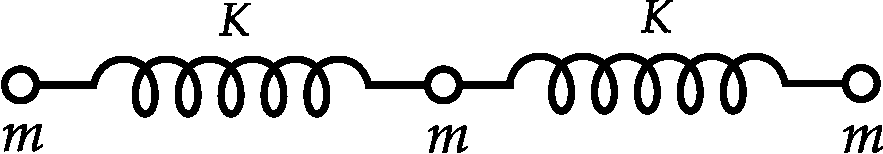
\includegraphics[height=1cm,width=5cm]{problem1}
		\end{figure}
		If $x_{1}, x_{2}$ and $x_{3}$ denote the horizontal displacement of the masses from their respective equilibrium positions the potential energy of the system is
		\exyear{NET DEC 2012}
	\end{minipage}
	\begin{tasks}(2)
		\task[\textbf{A.}] $\frac{1}{2} K\left[x_{1}^{2}+x_{2}^{2}+x_{3}^{2}\right]$
		\task[\textbf{B.}]$\frac{1}{2} K\left[x_{1}^{2}+x_{2}^{2}+x_{3}^{2}-x_{2}\left(x_{1}+x_{3}\right)\right]$
		\task[\textbf{C.}]$\frac{1}{2} K\left[x_{1}^{2}+2 x_{2}^{2}+x_{3}^{2}-2 x_{2}\left(x_{1}+x_{3}\right)\right]$
		\task[\textbf{D.}]$\frac{1}{2} K\left[x_{1}^{2}+2 x_{2}^{2}-2 x_{2}\left(x_{1}+x_{3}\right)\right]$
	\end{tasks}
	\begin{answer}
		\begin{align*}
		V&=\frac{1}{2} K\left(x_{2}-x_{1}\right)^{2}+\frac{1}{2} K\left(x_{3}-x_{2}\right)^{2}\\
		V&=\frac{1}{2} K\left(x_{2}^{2}+x_{1}^{2}-2 x_{2} x_{1}\right)+\frac{1}{2} K\left(x_{3}^{2}+x_{2}^{2}-2 x_{3} x_{2}\right)\\
		V&=\frac{1}{2} K\left[x_{1}^{2}+2 x_{2}^{2}+x_{3}^{2}-2 x_{2}\left(x_{1}+x_{3}\right)\right]
		\end{align*}
		The correct option is \textbf{(c)}
	\end{answer}
	\begin{minipage}{\textwidth}
		\item The time period of a simple pendulum under the influence of the acceleration due to gravity $g$ is $T$. The bob is subjected to an additional acceleration of magnitude $\sqrt{3} g$ in the horizontal direction. Assuming small oscillations, the mean position and time period of oscillation, respectively, of the bob will be
		\exyear{NET JUNE 2014}
	\end{minipage}
	\begin{tasks}(2)
		\task[\textbf{A.}] $0^{\circ}$ to the vertical and $\sqrt{3} T$
		\task[\textbf{B.}]$30^{\circ}$ to the vertical and $T / 2$
		\task[\textbf{C.}]$60^{\circ}$ to the vertical and $T / \sqrt{2}$
		\task[\textbf{D.}]$0^{\circ}$ to the vertical and $T / \sqrt{3}$
	\end{tasks}
	\begin{answer}
		\begin{align*}
		T&=2 \pi \sqrt{\frac{l}{g}}\\
		g^{\prime}&=\sqrt{3 g^{2}+g^{2}}=\sqrt{4 g^{2}}=2 g\\
		T^{\prime}&=2 \pi \sqrt{\frac{l}{2 g}} \Rightarrow T^{\prime}=2 \pi \sqrt{\frac{l}{g}} \cdot \frac{1}{\sqrt{2}} \Rightarrow T^{\prime}=\frac{T}{\sqrt{2}}\\
		T \cos \theta&=m g, T \sin \theta=\sqrt{3} m g \Rightarrow \tan \theta=\sqrt{3} \Rightarrow \theta=60^{\circ}
		\end{align*}
		The correct option is \textbf{(c)}	
	\end{answer}
	\begin{minipage}{\textwidth}
		\item A particle of mass $m$ is moving in the potential $V(x)=-\frac{1}{2} a x^{2}+\frac{1}{4} b x^{4}$ where $a, b$ are positive constants. The frequency of small oscillations about a point of stable equilibrium is
		\exyear{NET DEC 2014}
	\end{minipage}
	\begin{tasks}(2)
		\task[\textbf{A.}] $\sqrt{a / m}$
		\task[\textbf{B.}]$\sqrt{2 a / m}$
		\task[\textbf{C.}]$\sqrt{3 a / m}$
		\task[\textbf{D.}]$\sqrt{6 a / m}$
	\end{tasks}
	\begin{answer}
		\begin{align*}
		\because V(x)&=-\frac{1}{2} a x^{2}+\frac{1}{4} b x^{4}	\\
		\frac{\partial V}{\partial x}&=0 \Rightarrow-a x+b x^{3}=0 \Rightarrow x\left[-a+b x^{2}\right]=0 \Rightarrow x=\pm\left(\frac{a}{b}\right)^{\frac{1}{2}}, 0\\
		\because \frac{\partial^{2} V}{\partial x^{2}}&=-a+3 b x^{2}\\
		\text { At } x=0, \frac{\partial^{2} V}{\partial x^{2}}&=-a \text { (Negative so it is unstable point) }\\
		\left.\frac{\partial^{2} V}{\partial x^{2}}\right|_{x=\pm\left(\frac{a}{b}\right)^{\frac{1}{2}}}&=-a+3 b \frac{a}{b}=2 a \text { (Positive so it is stable point) }\\
		\Rightarrow \omega&=\sqrt{\frac{\frac{\partial^{2} V}{\partial x^{2}}}{m}}=\sqrt{\frac{2 a}{m}}
		\end{align*}
		The correct option is \textbf{(b)}
	\end{answer}
	\begin{minipage}{\textwidth}
		\item A particle of mass $m$, kept in potential $V(x)=-\frac{1}{2} k x^{2}+\frac{1}{4} \lambda x^{4}$ (where $k$ and $\lambda$ are positive constants), undergoes small oscillations about an equilibrium point. The frequency of oscillations is
		\exyear{NET JUNE 2018}
	\end{minipage}
	\begin{tasks}(2)
		\task[\textbf{A.}] $\frac{1}{2 \pi} \sqrt{\frac{2 \lambda}{m}}$
		\task[\textbf{B.}]$\frac{1}{2 \pi} \sqrt{\frac{k}{m}}$
		\task[\textbf{C.}]$\frac{1}{2 \pi} \sqrt{\frac{2 k}{m}}$
		\task[\textbf{D.}]$\frac{1}{2 \pi} \sqrt{\frac{\lambda}{m}}$
	\end{tasks}
	\begin{answer}
		\begin{align*}
		V&=-\frac{1}{2} k x^{2}+\frac{1}{4} \lambda x^{4}\\
		\frac{d V}{d x}&=0 \quad-k x+\lambda x^{3}=0\\
		x=0, \quad x^{2}&=\frac{k}{\lambda} \Rightarrow x=x_{0}=\sqrt{\frac{k}{\lambda}}\\
		\frac{d^{2} V}{d x^{2}}&=-k \quad \text { at } x=0 \quad \text { so } x=0 \text { is unstable part }\\
		\frac{d^{2} V}{d x^{2}}&=2 k \text { at } x_{0}=\sqrt{\frac{k}{\lambda}} \text { so } x_{0}=\sqrt{\frac{k}{x}} \text { is stable equation point }\\
		\omega&=\sqrt{\frac{\left.\frac{d^{2} V}{d x^{2}}\right|_{x=x_{0}}}{m}}=\sqrt{\frac{2 k}{m}} \quad f=\frac{1}{2 \pi} \sqrt{\frac{2 k}{m}}
		\end{align*}
		The correct option is \textbf{(c)}
	\end{answer}
\end{enumerate}